\documentclass[11pt]{article}
% =============================================================================
% preamble.tex — shared LaTeX preamble for the Pagesmith guides.
% \input this from each guide's .tex. Verified to compile with pdflatex (TeX Live).
% =============================================================================
\usepackage[margin=1in]{geometry}
\usepackage{amsmath,amssymb}
\usepackage{microtype}
\usepackage{enumitem}
\usepackage{xcolor}
\usepackage{hyperref}
\usepackage{listings}
\usepackage{tikz}
\usetikzlibrary{positioning,arrows.meta,shapes.geometric,calc,fit,backgrounds}
\usepackage{placeins}   % \FloatBarrier
\usepackage{caption}
\captionsetup{font=small,skip=8pt}

\hypersetup{colorlinks=true,linkcolor=blue!55!black,urlcolor=blue!55!black,citecolor=blue!55!black}

% A bit of breathing room around floats.
\setlength{\textfloatsep}{16pt plus 4pt minus 4pt}
\setlength{\intextsep}{16pt plus 4pt minus 4pt}

% ---- code listings ----------------------------------------------------------
\definecolor{codebg}{RGB}{248,248,248}
\definecolor{codecmt}{RGB}{0,128,0}
\definecolor{codestr}{RGB}{170,55,0}
\definecolor{codekw}{RGB}{0,0,180}
% No fixed `language=` (so neither JS nor JSON trips listings' keyword parser);
% code is shown as clean monospace in a framed, tinted box.
\lstset{
  basicstyle=\ttfamily\small,
  backgroundcolor=\color{codebg},
  commentstyle=\color{codecmt}\itshape,
  stringstyle=\color{codestr},
  showstringspaces=false,
  breaklines=true,
  columns=fullflexible,
  keepspaces=true,
  frame=single,
  framesep=4pt,
  rulecolor=\color{black!20},
  aboveskip=10pt,
  belowskip=6pt
}

% ---- tikz diagram helpers (boxes + arrows) ----------------------------------
\definecolor{boxblue}{RGB}{79,124,255}
\definecolor{boxgray}{RGB}{90,98,112}
\tikzset{
  box/.style   = {draw, rounded corners, align=center, font=\small, inner sep=6pt, fill=boxblue!8, draw=boxblue!60},
  gbox/.style  = {draw, rounded corners, align=center, font=\small, inner sep=6pt, fill=black!4, draw=black!35},
  flow/.style  = {-{Stealth[length=2.4mm]}, thick, draw=boxgray},
}

% ---- convenience macros -----------------------------------------------------
\newcommand{\code}[1]{\texttt{#1}}


\title{Pagesmith --- The Skeleton \& Catalogue\\[2pt]\large A Developer Guide to the Engine}
\author{David Falk}
\date{}

\begin{document}
\maketitle

\begin{abstract}
\noindent Pagesmith is a generic, JSON-driven page-builder engine written in
plain, dependency-free JavaScript. This guide explains how that engine works end
to end, for a developer who wants to build on or extend it. We cover the
philosophy (longevity, the engine-versus-instance split), the data model (a page
is a flat array of typed blocks in a JSON file), the boot and load order, the
event-driven render data-flow, and --- the centrepiece --- \emph{the catalogue
and the part contract}: how to write a self-contained component and the rules it
must obey so it composes with every other part and stays portable across sites.
We finish with the editing protocol, the two namespaces, theming, the
shape-generic backend, and a checklist for standing up a new site. The deep
internals of the inline editor are a separate guide; this one documents the
producer side a part author needs.
\end{abstract}

\tableofcontents
\bigskip

%==============================================================================
\section{Philosophy: why it is built this way}
%==============================================================================

Before any code, it is worth understanding \emph{why} Pagesmith looks the way it
does, because every decision downstream falls out of three commitments.

\subsection{Plain, dependency-free JavaScript}

There is no framework here. No React, no Vue, no build step, no
\code{npm install} on the front end, no bundler, no transpiler. Every file under
\code{app/javascript/} is an IIFE --- an old-fashioned
\code{(function () \{ ... \})()} --- that runs directly in the browser exactly as
written. The catalogue builds DOM with \code{document.createElement}. State lives
in a JSON file. Events are plain \code{CustomEvent}s.

This is a deliberate, almost stubborn choice, and the reason is
\textbf{longevity}. A framework is a bet that a particular toolchain will still
be installable, patchable, and well-understood in five or ten years. That bet
frequently loses: the build breaks, a transitive dependency is abandoned, a major
version forces a rewrite. Plain JavaScript served as static files has no such
failure mode. If a browser can run it today, it will run it in a decade. The cost
is that you write a little more by hand; the payoff is that the thing keeps
working with zero maintenance. For a tool whose whole job is to outlive the
attention span of whoever set it up, that trade is the entire point.

\begin{quote}
\small\emph{Aside.} You will notice the code is written in a conservative
dialect: \code{var} not \code{let}, \code{function} expressions in the hot paths,
\code{[].forEach.call(...)} for NodeLists. That is not nostalgia --- it is the
same longevity instinct. The fewer language features you lean on, the fewer ways
the floor can move under you.
\end{quote}

\subsection{The engine-versus-instance split}

Pagesmith is two halves that never blur into each other (Figure~\ref{fig:split}).
The \textbf{engine} knows \emph{nothing} about your site --- not its name,
colours, pages, or social links. It reads all of that from the \textbf{instance}
at runtime. The contract is strict and one-directional: the instance depends on
the engine; the engine never depends on the instance. The single bridge is
\code{site-config.js}, a plain manifest of values, plus the optional
\code{site-blocks.js}, where you register parts that only make sense for one site.

\begin{figure}[h]
\centering
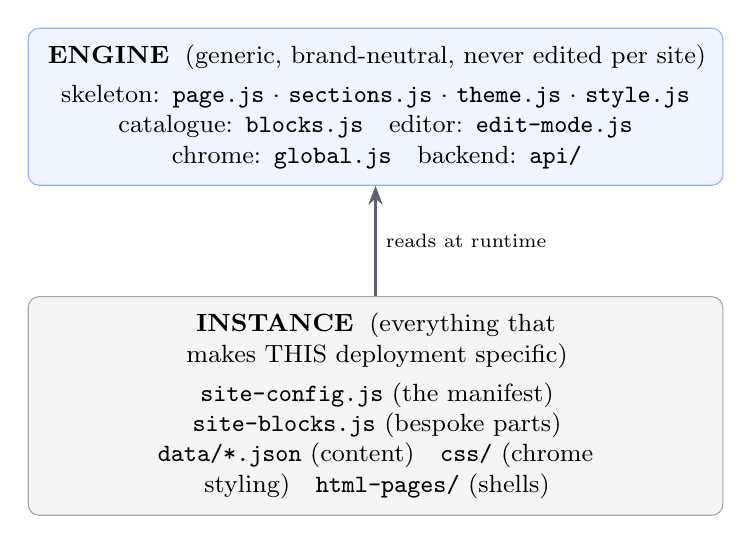
\begin{tikzpicture}[node distance=6mm]
  \node[box, text width=8.4cm] (eng) {\textbf{ENGINE} \;(generic, brand-neutral, never edited per site)\\[3pt]
    skeleton: \code{page.js} $\cdot$ \code{sections.js} $\cdot$ \code{theme.js} $\cdot$ \code{style.js}\\
    catalogue: \code{blocks.js}\quad editor: \code{edit-mode.js}\\
    chrome: \code{global.js}\quad backend: \code{api/}};
  \node[gbox, below=14mm of eng, text width=8.4cm] (inst) {\textbf{INSTANCE} \;(everything that makes THIS deployment specific)\\[3pt]
    \code{site-config.js} (the manifest)\quad \code{site-blocks.js} (bespoke parts)\\
    \code{data/*.json} (content)\quad \code{css/} (chrome styling)\quad \code{html-pages/} (shells)};
  \draw[flow] (inst) -- node[right, font=\scriptsize]{reads at runtime} (eng);
\end{tikzpicture}
\caption{The one-directional dependency. The instance reads the engine; the
engine never reads the instance.}
\label{fig:split}
\end{figure}

The reason this matters is \textbf{reuse without forking}. Because the engine
carries no site-specific strings, the same battle-tested files drop into any
number of sites unchanged. Bug fixes and new parts flow to every site by copying
engine files; nothing site-specific ever has to be untangled first. To stand up a
new site you change values, not code.

\begin{quote}
\small\emph{The litmus test for ``does this belong in the engine?''} If a line of
code mentions a brand, a colour by name, a specific page, or a specific URL, it
is \emph{instance}, and it belongs in \code{site-config.js} /
\code{site-blocks.js} / \code{data/}. The engine deals only in \emph{roles} and
\emph{shapes}.
\end{quote}

%==============================================================================
\section{The data model: a page is a JSON file}
%==============================================================================

This is the keystone, so go slowly. \textbf{A page is a JSON file.} That is the
whole model. A page lives at \code{data/page-<slug>.json} and has this shape:

\begin{lstlisting}
{
  "title": "Showcase",
  "theme": { "accent": "#ff3b8e" },
  "sections": [
    { "id": "sc-h",     "type": "heading", "visible": true, "text": "Component showcase" },
    { "id": "sc-intro", "type": "text",    "title": "The catalogue",
      "body": "These are the building blocks Pagesmith ships with." }
  ]
}
\end{lstlisting}

Three top-level keys, and only \code{sections} is required: \code{title}
(optional, sets the tab title), \code{theme} (optional, a per-page colour
override; absent $\rightarrow$ inherit the site default from \code{global.json}),
and \code{sections} --- an \textbf{ordered, flat array of typed blocks}, which
\emph{is} the page.

\subsection{Blocks are flat and typed}

Every entry in \code{sections[]} is a \textbf{block}: a plain object whose
\code{type} names a part in the catalogue, plus whatever data that part needs. The
engine guarantees each block an \emph{envelope} of fields, filling them in if
absent (\code{normalize()} in \code{blocks.js}):

\begin{center}\small
\begin{tabular}{ll}
\hline
\textbf{Field} & \textbf{Meaning}\\
\hline
\code{id}      & stable identifier; the editor keys reorder/hide/remove on it\\
\code{type}    & which catalogue part renders it; unknown $\rightarrow$ falls back to \code{text}\\
\code{visible} & \code{false} hides the block on the published page\\
\code{style}   & optional per-block inline styling (see \code{style.js})\\
\hline
\end{tabular}
\end{center}

Everything \emph{else} on the block is part-specific payload: a \code{gallery}
carries \code{images:[...]}; a \code{chart} carries \code{kind} and
\code{series:[...]}; a \code{spotlight} carries \code{value}/\code{label}/%
\code{caption}. The engine does not care --- it hands the whole block to the part
and lets the part read what it needs.

\begin{quote}
\small\emph{Why flat, not a tree?} A flat array is trivial to reason about,
reorder (just array-index manipulation), diff, and store. Nesting \emph{is}
supported --- the \code{group} part holds a \code{children:[...]} array and
renders it recursively --- but nesting is opt-in, owned by one part, rather than
baked into the model. The model stays a list; complexity lives in the parts that
want it.
\end{quote}

The shared site chrome (header, footer, nav, social, theme default) lives in one
more file of the same family, \code{data/global.json}. It is not a page (no
\code{sections[]}) but flows through the very same machinery (see \code{global.js}
and Section~\ref{sec:flow}).

%==============================================================================
\section{Boot and load order}
%==============================================================================

A page is an almost-empty HTML shell (\code{html-pages/page.html}): a
\code{<main></main>} and little else, with \emph{no} per-page CSS or JS. The body
is built entirely from \code{sections[]} at runtime. So: what scripts load, in
what order, and why does order matter?

The \code{<head>} loads two scripts synchronously: \code{site-config.js} then
\code{media-base.js}. \textbf{\code{site-config.js} is first, always.} It defines
\code{window.SITE\_CONFIG} and the read-only accessor \code{window.SITE}. Being
synchronous and first, \code{window.SITE} is guaranteed to exist before any other
engine code runs --- which matters because the very next script,
\code{media-base.js}, already asks \code{SITE.isProd(host)} to decide whether to
load the editor and which storage container to read.

\textbf{\code{media-base.js} is the bootstrapper.} It patches \code{window.fetch}
(redirecting \code{/data/X.json} to the right blob container, and rewriting
\code{/media-content/...} references to real storage URLs everywhere --- JSON
bodies, DOM attributes, CSS rules --- via a \code{MutationObserver}), and then
\emph{injects the rest of the engine in a deliberate order}
(Figure~\ref{fig:load}).

\begin{figure}[h]
\centering
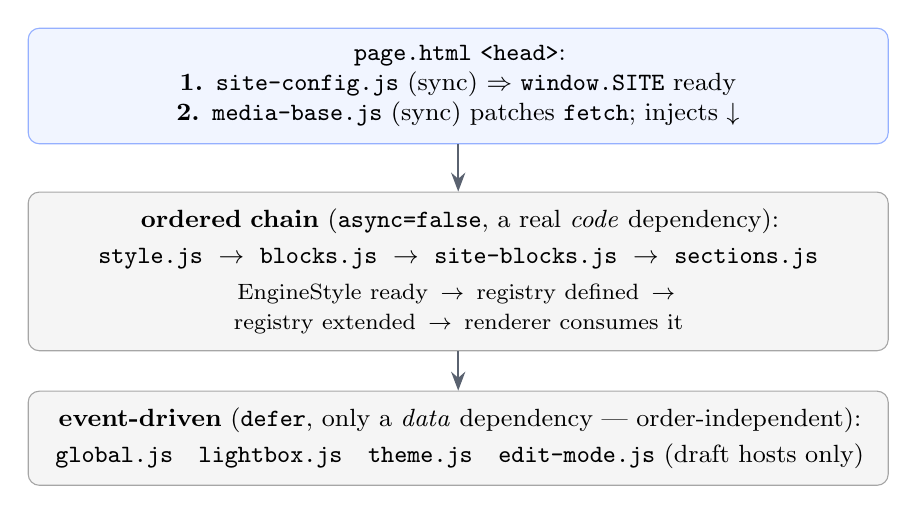
\begin{tikzpicture}[node distance=4mm]
  \node[box, text width=10.5cm] (head) {\code{page.html} \code{<head>}:\\
    \textbf{1.} \code{site-config.js} (sync) $\Rightarrow$ \code{window.SITE} ready\quad
    \textbf{2.} \code{media-base.js} (sync) patches \code{fetch}; injects $\downarrow$};
  \node[gbox, below=6mm of head, text width=10.5cm] (chain) {\textbf{ordered chain} (\code{async=false}, a real \emph{code} dependency):\\[2pt]
    \code{style.js} \;$\rightarrow$\; \code{blocks.js} \;$\rightarrow$\; \code{site-blocks.js} \;$\rightarrow$\; \code{sections.js}\\[2pt]
    \footnotesize EngineStyle ready $\,\rightarrow\,$ registry defined $\,\rightarrow\,$ registry extended $\,\rightarrow\,$ renderer consumes it};
  \node[gbox, below=5mm of chain, text width=10.5cm] (evt) {\textbf{event-driven} (\code{defer}, only a \emph{data} dependency --- order-independent):\\[2pt]
    \code{global.js}\quad \code{lightbox.js}\quad \code{theme.js}\quad \code{edit-mode.js} (draft hosts only)};
  \draw[flow] (head) -- (chain);
  \draw[flow] (chain) -- (evt);
\end{tikzpicture}
\caption{Load order. The catalogue chain uses ordered execution; theming and
chrome use events.}
\label{fig:load}
\end{figure}

Two mechanisms are at work, doing different jobs:

\begin{enumerate}[leftmargin=1.4em]
\item \textbf{Ordered execution} (\code{async=false}) for
\code{style.js}\,$\rightarrow$\,\code{blocks.js}\,$\rightarrow$\,%
\code{site-blocks.js}\,$\rightarrow$\,\code{sections.js}. Injected scripts
default to \code{async} (``run whenever downloaded'' --- a race); setting
\code{async=false} forces execution in insertion order regardless of download
timing. This yields a strict dependency chain: \code{style.js} publishes
\code{EngineStyle} (the catalogue calls \code{EngineStyle.apply()} on render);
\code{blocks.js} defines the registry \code{window.Catalog}; \code{site-blocks.js}
runs after it and adds to it; \code{sections.js} runs last, so the full registry
(generic + bespoke) exists before it renders.
\item \textbf{Event-driven} (\code{defer}) for everything else. \code{global.js}
and \code{theme.js} do not care \emph{when} they load relative to \code{page.js},
because they listen for \code{engine-data-ready} (with a fallback for the case
where the event already fired).
\end{enumerate}

\begin{quote}
\small\emph{Why two mechanisms?} The catalogue chain has a real \emph{code}
dependency (\code{sections.js} literally calls \code{Catalog.render}), so it needs
hard ordering. Theming and chrome only have a \emph{data} dependency, so they use
events and become order-independent --- more robust than ordering everything.
\end{quote}

%==============================================================================
\section{The render data-flow}
\label{sec:flow}
%==============================================================================

Now the heart: how data becomes DOM. The flow is \textbf{event-driven and
order-independent} (Figure~\ref{fig:dataflow}).

\begin{figure}[h]
\centering
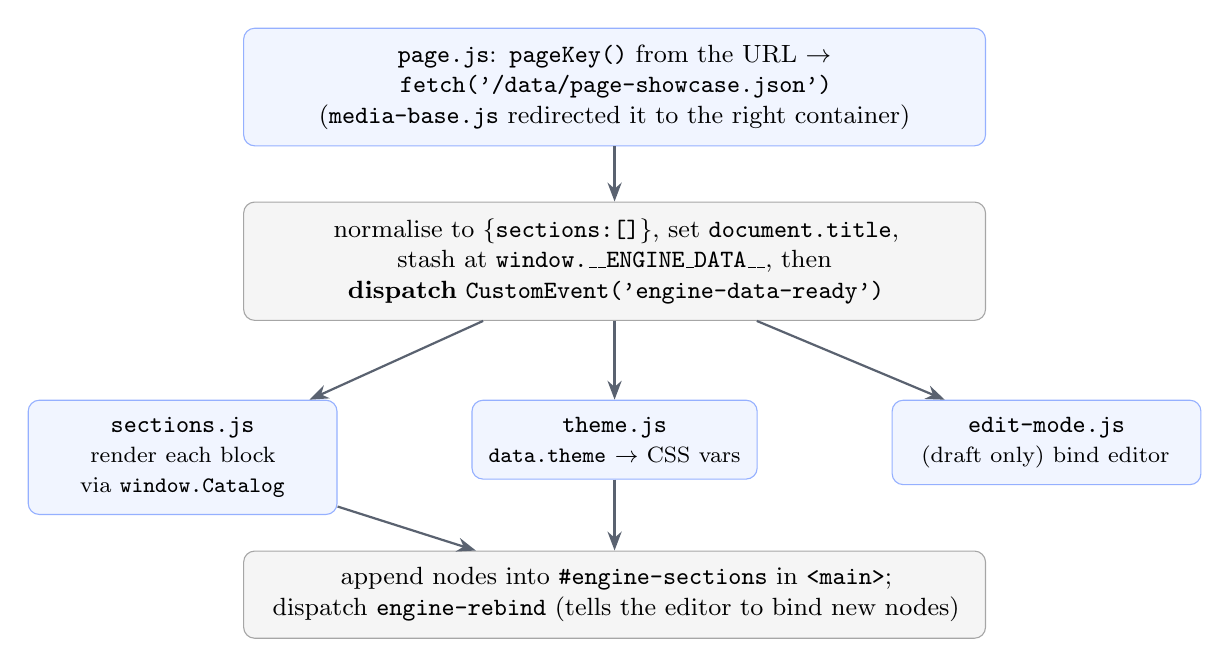
\begin{tikzpicture}[node distance=7mm]
  \node[box, text width=9cm] (pg) {\code{page.js}: \code{pageKey()} from the URL $\rightarrow$
    \code{fetch('/data/page-showcase.json')}\\(\code{media-base.js} redirected it to the right container)};
  \node[gbox, below=7mm of pg, text width=9cm] (ann) {normalise to \code{\{sections:[]\}}, set \code{document.title},\\
    stash at \code{window.\_\_ENGINE\_DATA\_\_}, then\\
    \textbf{dispatch} \code{CustomEvent('engine-data-ready')}};
  \node[box, below left=10mm and -1.2cm of ann, text width=3.5cm] (sec) {\code{sections.js}\\\footnotesize render each block via \code{window.Catalog}};
  \node[box, below=10mm of ann, text width=3.2cm] (th) {\code{theme.js}\\\footnotesize \code{data.theme} $\rightarrow$ CSS vars};
  \node[box, below right=10mm and -1.2cm of ann, text width=3.5cm] (ed) {\code{edit-mode.js}\\\footnotesize (draft only) bind editor};
  \node[gbox, below=9mm of th, text width=9cm] (out) {append nodes into \code{\#engine-sections} in \code{<main>};\\
    dispatch \code{engine-rebind} (tells the editor to bind new nodes)};
  \draw[flow] (pg) -- (ann);
  \draw[flow] (ann) -- (sec);
  \draw[flow] (ann) -- (th);
  \draw[flow] (ann) -- (ed);
  \draw[flow] (sec) -- (out);
  \draw[flow] (th) -- (out);
\end{tikzpicture}
\caption{The render data-flow. \code{page.js} \emph{announces}; \code{sections.js},
\code{theme.js}, and the editor each \emph{react}.}
\label{fig:dataflow}
\end{figure}

Concretely: \code{page.js} runs on \code{DOMContentLoaded}. \code{pageKey()}
derives a content-file key from the URL in priority order --- an explicit
\code{<meta name="engine-page">}, then a \code{/p/<slug>} route, then a clean
top-level slug, defaulting to \code{home} --- sanitising the slug to
\code{[a-z0-9-]} so the filename can never traverse out of \code{/data/}. It then
fetches \code{/data/<key>.json}. A missing file is \emph{not} an error: a
brand-new page has no JSON yet, so a 404 becomes an empty page the editor can
fill. \code{page.js} normalises the data, sets the title, stashes it on
\code{window.\_\_ENGINE\_DATA\_\_}, and fires \code{engine-data-ready}.

That event is the linchpin. \code{page.js} does not \emph{call} the renderer or
themer; it \emph{announces} the data and lets anyone interested react. Each
listener also checks \code{window.\_\_ENGINE\_DATA\_\_} on startup, to catch the
case where the event fired \emph{before} the listener attached. This is the
order-independence in action: the load order can shuffle and the page still
composes.

\code{sections.js} is intentionally ignorant --- it never hard-codes a block
type. For each entry it builds a small \code{ctx} and calls
\code{window.Catalog.render(block, ctx)}, appending the node into
\code{\#engine-sections}. New part types appear with \emph{zero} changes here.
When done it fires \code{engine-rebind} so the editor can bind the new nodes.

\begin{quote}
\small\emph{Note on \code{global.json}.} The shared chrome flows through the
\emph{same} event: \code{global.js} fetches it, hydrates header/footer, and
dispatches \code{engine-data-ready} with \code{file:'global'}. \code{sections.js}
ignores that one (global is chrome, not a page); \code{theme.js} applies its
theme as the site-wide default before a page's own theme overrides it.
\end{quote}

%==============================================================================
\section{The catalogue and the part contract}
\label{sec:catalogue}
%==============================================================================

This is the centrepiece. The catalogue (\code{blocks.js}) is a \textbf{registry
of part types}. Each entry is a fully self-contained component bundling four
things that a framework would scatter across files: its \textbf{markup} (a
\code{render()} returning a DOM node), its \textbf{styling} (CSS injected once,
namespaced \code{catalog-}), its \textbf{edit schema}
(\code{fields[]}/\code{lists\{\}} the editor reads), and its \textbf{behaviour}
(an optional \code{init()}). Adding a capability to the \emph{entire system} ---
a section anyone can add, that edits, themes, and persists --- is adding one
object to this registry. That containment is what makes the engine portable.

\subsection{Anatomy of a part}

\begin{figure}[h]
\centering
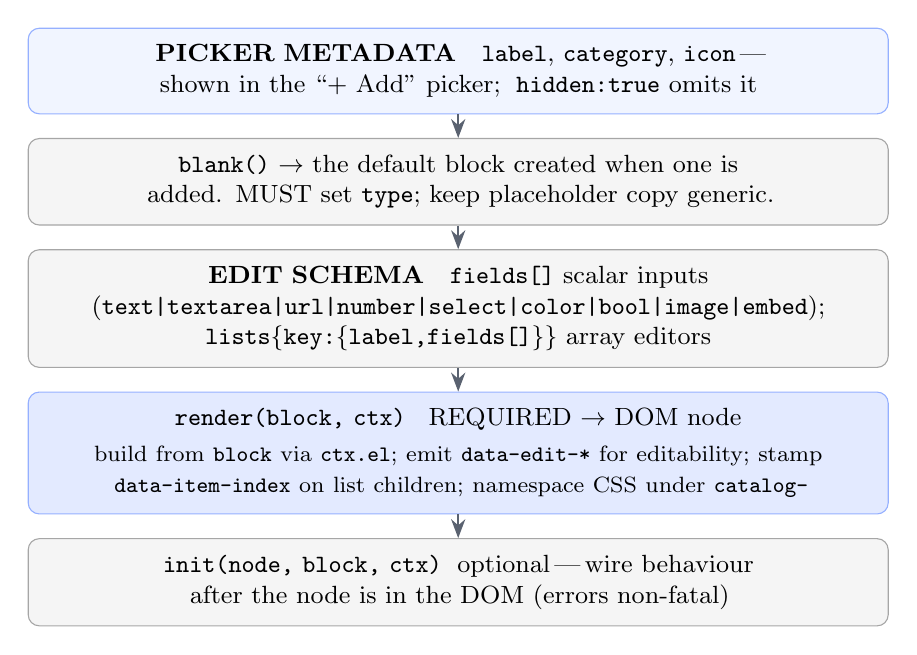
\begin{tikzpicture}[node distance=3mm]
  \node[box, text width=10.5cm] (meta) {\textbf{PICKER METADATA}\quad
    \code{label}, \code{category}, \code{icon}\,---\,shown in the ``+ Add'' picker;\;
    \code{hidden:true} omits it};
  \node[gbox, below=3mm of meta, text width=10.5cm] (blank) {\code{blank()} $\rightarrow$ the default block created when one is added.
    MUST set \code{type}; keep placeholder copy generic.};
  \node[gbox, below=3mm of blank, text width=10.5cm] (schema) {\textbf{EDIT SCHEMA}\quad
    \code{fields[]} scalar inputs (\code{text|textarea|url|number|select|color|bool|image|embed});\;
    \code{lists\{key:\{label,fields[]\}\}} array editors};
  \node[box, below=3mm of schema, text width=10.5cm, fill=boxblue!16] (render) {\textbf{\code{render(block, ctx)}} \;\;REQUIRED $\rightarrow$ DOM node\\[2pt]
    \footnotesize build from \code{block} via \code{ctx.el}; emit \code{data-edit-*} for editability;
    stamp \code{data-item-index} on list children; namespace CSS under \code{catalog-}};
  \node[gbox, below=3mm of render, text width=10.5cm] (init) {\code{init(node, block, ctx)} \;optional\,---\,wire behaviour after the node is in the DOM (errors non-fatal)};
  \draw[flow] (meta) -- (blank);
  \draw[flow] (blank) -- (schema);
  \draw[flow] (schema) -- (render);
  \draw[flow] (render) -- (init);
\end{tikzpicture}
\caption{Anatomy of a part: every key a registry entry may define.}
\label{fig:part}
\end{figure}

\subsection{The \code{ctx} object}

Every \code{render(block, ctx)} (and \code{init}) receives a small context built
by the renderer. It is the part's entire window onto the engine:

\begin{center}\small
\begin{tabular}{lp{8.4cm}}
\hline
\textbf{\code{ctx} key} & \textbf{What it is / why you need it}\\
\hline
\code{ctx.el} & tiny DOM builder \code{el(tag, attrs, kids)}; \code{text}/\code{html} are special-cased, all else becomes an attribute\\
\code{ctx.mediaUrl} & resolves a \code{/media-content/...} path to the real (blob/local) URL so your \code{<img src>} works everywhere\\
\code{ctx.file} & the content-file key (e.g. \code{page-showcase}); goes into \code{data-edit-file}\\
\code{ctx.index} & this block's index in \code{sections[]}; handy for unique ids (e.g. a chart gradient) and lightbox grouping\\
\code{ctx.path} & the data-path to this block, e.g.\ \code{sections[2]} --- \textbf{the base for every \code{data-edit-*} path you emit}\\
\hline
\end{tabular}
\end{center}

The \code{block} argument is just the block's data --- the same object that sat in
the JSON \code{sections[]}.

\subsection{Two real parts, read closely}

The smallest useful part --- \code{text}:

\begin{lstlisting}
text: {
  label: 'Text', category: 'Basic', icon: '|P|',
  blank: function () { return { type: 'text', title: 'New section', body: 'Add your text here.' }; },
  render: function (block, ctx) {
    var sec = ctx.el('section', { 'class': 'engine-section' });
    sec.appendChild(ctx.el('h2', {
      'class': 'engine-section-title', text: block.title || '',
      'data-edit-file': ctx.file, 'data-edit-text': ctx.path + '.title'
    }));
    sec.appendChild(ctx.el('div', {
      'class': 'engine-section-body', html: block.body || '',
      'data-edit-file': ctx.file, 'data-edit-html': ctx.path + '.body'
    }));
    return sec;
  }
}
\end{lstlisting}

What makes the title and body \emph{editable} is nothing more than the
\code{data-edit-file} + \code{data-edit-text}/\code{data-edit-html} pairs, with
the path built off \code{ctx.path}. The part author writes no editor code.

A list-bearing part --- \code{gallery} --- adds a \code{lists\{\}} schema and
stamps \code{data-item-index} on each child:

\begin{lstlisting}
gallery: {
  label: 'Photo gallery', category: 'Media', icon: '[#]',
  blank: function () { return { type: 'gallery', title: 'New gallery', images: [] }; },
  lists: { images: { label: 'Image', fields: [
    { key: 'src', type: 'image', label: 'Image' },
    { key: 'alt', type: 'text',  label: 'Alt text' }
  ] } },
  render: function (block, ctx) {
    var sec  = ctx.el('section', { 'class': 'engine-section' });
    var grid = ctx.el('div', { 'class': 'engine-gallery',
      'data-edit-file': ctx.file,
      'data-edit-list': ctx.path + '.images',
      'data-edit-list-label': 'images' });
    (Array.isArray(block.images) ? block.images : []).forEach(function (im, j) {
      var src = (im && im.src) ? im.src : '';
      grid.appendChild(ctx.el('img', {
        src: ctx.mediaUrl(src), alt: (im && im.alt) || '', loading: 'lazy',
        'data-item-index': j,                        // TRUE array index
        'data-edit-file': ctx.file,
        'data-edit-image': ctx.path + '.images[' + j + '].src'
      }));
    });
    sec.appendChild(grid); return sec;
  }
}
\end{lstlisting}

The container carries \code{data-edit-list} (so the editor's list machinery binds
to it); each child carries an editable path and its true \code{data-item-index}.
The \code{Array.isArray(...)} guard means a malformed \code{images} degrades to an
empty grid instead of throwing.

\subsection{How the renderer drives a part}

\code{renderOne(block, ctx)} is the only thing that calls your part, in a fixed
sequence worth knowing because it tells you what is guaranteed when your code
runs:

\begin{enumerate}[leftmargin=1.6em, itemsep=1pt]
\item \code{ensureCSS()} --- inject the catalogue stylesheet once (lazy, idempotent);
\item refresh \code{STATPAL} from the live \code{--cat-*} palette (theming current);
\item look up \code{BLOCKS[block.type]}, falling back to \code{text} for unknown types;
\item call your \code{render(block, ctx)} to get a node;
\item stamp engine bookkeeping: \code{data-engine-block}, \code{data-engine-index}, \code{data-engine-path};
\item apply block \code{style} and per-text \code{textStyles} via \code{EngineStyle};
\item call your \code{init(node, block, ctx)} inside a \code{try/catch} --- a throw is non-fatal.
\end{enumerate}

\subsection{Worked example: adding a part to \code{site-blocks.js}}

\code{site-blocks.js} ships empty, with a commented template. Here is the full
procedure to add a bespoke \code{hero}. Everything goes inside the file's IIFE.

\begin{lstlisting}
(function () {
  'use strict';
  if (!window.CatalogBlocks) return;   // engine not loaded -> no-op, never throw

  window.CatalogBlocks['hero'] = {
    label: 'Hero', category: 'Layout', icon: '*',          // 2. picker metadata
    blank: function () {                                    // 3. default block; MUST set type
      return { type: 'hero', title: 'Big headline', subtitle: 'Supporting line' };
    },
    fields: [                                              // 4. inspector inputs
      { key: 'title',    type: 'text', label: 'Headline' },
      { key: 'subtitle', type: 'text', label: 'Subtitle' }
    ],
    render: function (block, ctx) {                        // 5. build DOM + data-edit-*
      ensureHeroCSS();
      var sec = ctx.el('section', { 'class': 'engine-section catalog-hero' });
      sec.appendChild(ctx.el('h1', { 'class': 'catalog-hero-title',
        text: block.title || '',
        'data-edit-file': ctx.file, 'data-edit-text': ctx.path + '.title' }));
      sec.appendChild(ctx.el('p', { 'class': 'catalog-hero-sub',
        text: block.subtitle || '',
        'data-edit-file': ctx.file, 'data-edit-text': ctx.path + '.subtitle' }));
      return sec;
    }
  };

  function ensureHeroCSS() {                               // 6. inject CSS once, namespaced, themed
    if (document.getElementById('catalog-hero-styles')) return;
    var s = document.createElement('style');
    s.id = 'catalog-hero-styles';
    s.textContent = [
      '.catalog-hero{text-align:center;padding:3rem 1rem}',
      '.catalog-hero-title{font-size:clamp(2rem,6vw,4rem);margin:0;color:var(--site-ink,#fff)}',
      '.catalog-hero-sub{opacity:.8;margin:.6rem 0 0;color:var(--site-ink,#fff)}'
    ].join('\n');
    document.head.appendChild(s);
  }
})();
\end{lstlisting}

\textbf{Step 7 --- that's it.} Reload a draft page. The \code{hero} appears in the
picker, can be added, its text is click-to-edit on the page \emph{and} editable
from the inspector, its styling is namespaced and theme-aware, and Save persists
it like any other block. You wrote one object and one CSS helper --- no changes
to \code{sections.js}, \code{page.js}, the editor, or the backend. If your part
needs runtime behaviour, add \code{init}; if it has an array, add a
\code{lists\{\}} schema and stamp \code{data-item-index} per child, exactly like
\code{gallery}.

%==============================================================================
\section{The rules every part must follow}
\label{sec:rules}
%==============================================================================

A part is portable and composable only if it obeys a handful of rules. Treat this
as a checklist. Each rule exists because violating it breaks composition with
\emph{other} parts, or portability across \emph{other} sites.

\begin{itemize}[leftmargin=1.4em, itemsep=3pt]
\item[$\square$] \textbf{Namespace every CSS class under \code{catalog-}.} Class
names like \code{.catalog-hero-title}, not \code{.title}. \emph{(Two parts on one
page, or one part on a foreign site, must not leak styles into each other.)}
\item[$\square$] \textbf{Inject CSS once, lazily, on first render.} Guard with a
unique \code{id} and append a single \code{<style>}. \emph{(A part must look right
on any page, and must not re-inject for each instance.)}
\item[$\square$] \textbf{Emit \code{data-edit-*} for everything editable.} Text
$\rightarrow$ \code{data-edit-text}; rich text $\rightarrow$ \code{data-edit-html};
images $\rightarrow$ \code{data-edit-image}; arrays $\rightarrow$
\code{data-edit-list}; an attribute $\rightarrow$ \code{data-edit-attr}; always
pair with \code{data-edit-file}. \emph{(The only way the generic editor can edit
your part.)}
\item[$\square$] \textbf{Build paths off \code{ctx.path}.} Never hard-code
\code{sections[2]}; use \code{ctx.path + '.title'}. \emph{(The same part renders at
different indices and inside groups at deep paths like
\code{sections[1].children[0]}.)}
\item[$\square$] \textbf{Stamp \code{data-item-index} on every list child} ---
its \emph{true} array index. \emph{(On-page drag reorders the right item even when
some items are filtered out of the render.)}
\item[$\square$] \textbf{Guard with \code{Array.isArray}/falsy checks ---
degrade, never throw.} \emph{(Content can be partial mid-edit; a part that throws
takes the whole render down, a part that degrades shows an empty-but-valid
section.)}
\item[$\square$] \textbf{Be theme-aware via CSS variables} ---
\code{var(--site-accent, ...)}, \code{var(--cat-1, ...)}, always with a fallback.
\emph{(A theme change in JSON must re-colour your part with no code edit; the
fallback keeps it good with no theme at all.)}
\item[$\square$] \textbf{No site-specific strings in \code{blocks.js}} --- brands,
real pages, real URLs belong in \code{site-blocks.js} or content.
\emph{(\code{blocks.js} is engine; it must drop into any site unchanged.)}
\end{itemize}

\begin{quote}
\small\emph{The unifying idea.} Every rule is a corollary of one principle: a part
is a black box that talks to the engine only through the documented contract (the
registry keys, \code{ctx}, \code{data-edit-*}, the CSS variables) and otherwise
keeps entirely to itself. Stay inside that boundary and your part composes with
every other part and travels to every other site.
\end{quote}

%==============================================================================
\section{The editing protocol}
%==============================================================================

You make a part editable purely by tagging its DOM. The editor
(\code{edit-mode.js}, documented fully in the separate \emph{Editor --- Developer
Guide}) scans for these attributes and wires the interactions. As a part author
you need only the producer side:

\begin{center}\small
\begin{tabular}{lll}
\hline
\textbf{Attribute (with \code{data-edit-file})} & \textbf{Makes editable} & \textbf{Example value}\\
\hline
\code{data-edit-text}  & plain text of the node      & \code{sections[2].title}\\
\code{data-edit-html}  & rich text (innerHTML)       & \code{sections[2].body}\\
\code{data-edit-image} & an image (opens the picker) & \code{sections[2].images[0].src}\\
\code{data-edit-attr}  & one attribute, \code{path|attr} & \code{sections[2].url|href}\\
\code{data-edit-bg}    & a background image          & \code{sections[2].style.bgImage}\\
\code{data-edit-list}  & a reorderable array         & \code{sections[2].images}\\
\code{data-item-index} & (on each list child) its index & \code{0}, \code{1}, \code{2}\\
\hline
\end{tabular}
\end{center}

Every value is a \textbf{data-path}: a dotted/bracketed address into the page
JSON, such as \code{sections[2].items[0].value}. The editor resolves the path,
edits that spot in the in-memory data, re-renders, and on Save writes the JSON
back. You never write that resolution code --- you only emit the right path, and
you always build it from \code{ctx.path} so it is correct at any depth. The deep
editor internals are covered in the \emph{Editor --- Developer Guide}; cross-refer
it when you need the consumer side.

%==============================================================================
\section{The two namespaces: \texttt{engine-} vs \texttt{catalog-}}
%==============================================================================

Pagesmith uses exactly two prefixes, and the split is meaningful:

\begin{center}\small
\begin{tabular}{lp{8.6cm}}
\hline
\textbf{Prefix} & \textbf{Owns}\\
\hline
\code{engine-} & the skeleton, editor, and page structure: \code{.engine-section},
\code{\#engine-sections}, \code{window.EngineStyle}/\code{EngineTheme}/%
\code{EngineEdit}, the \code{engine-data-ready}/\code{engine-rebind} events,
\code{data-engine-path}\\
\code{catalog-} & the parts: \code{.catalog-carousel}, \code{.catalog-statcard},
\code{.catalog-hero}, \code{window.Catalog}, \code{window.CatalogBlocks}\\
\hline
\end{tabular}
\end{center}

The reason for two namespaces is the engine-versus-instance /
skeleton-versus-parts boundary \emph{made visible}. Anything \code{engine-} is
structural plumbing owned by the skeleton and editor: stable, rarely touched.
Anything \code{catalog-} is a part's own surface: parts may be added, removed, or
replaced freely. Reading a stylesheet or a stack trace, the prefix instantly
tells you which layer you are in and which rules apply --- \code{engine-} classes
are shared and must not be reused by parts; \code{catalog-} classes belong to one
part and must not collide with another.

%==============================================================================
\section{Theming}
%==============================================================================

Colour and brand are kept \emph{out of the code} and expressed as CSS custom
properties. The engine and every part reference variables like
\code{var(--site-accent)}; \code{theme.js} is the one place that sets them, from
data. It reads a \code{theme} object --- from \code{global.json} (site default)
and/or a page's own JSON (override) --- and writes the matching variables onto
\code{<html>}. It is event-driven: \code{global.json}'s theme sets the defaults; a
page's theme arrives after and overrides.

\begin{center}\small
\begin{tabular}{lll}
\hline
\textbf{\code{theme} key} & \textbf{CSS variable} & \textbf{Role}\\
\hline
\code{accent}        & \code{--site-accent}           & links, buttons, chart bars\\
\code{text}          & \code{--site-ink}              & main foreground / ink\\
\code{bg}            & \code{--site-bg}               & page background colour\\
\code{palette:[..]}  & \code{--cat-1}\,\dots\,\code{--cat-N} & data-viz palette\\
\code{spotlight}     & \code{--cat-spot}              & the spotlight gradient\\
\code{bgImage}       & \code{--site-bg-image}         & full-bleed background photo\\
\hline
\end{tabular}
\end{center}

Two details worth internalising. \textbf{Clearing reverts live:} when a
\code{theme} key is absent, \code{theme.js} actively \code{removeProperty()}s the
variable rather than skipping it, so deleting a colour in the editor immediately
falls back to the stylesheet default. \textbf{\code{--cat-*} is overridable but
optional:} parts read the palette via \code{STATPAL = palette()}, which pulls
\code{--cat-1..8} from the live computed style and falls back to a built-in neon
default, so the catalogue looks good with no theme \emph{and} a site can recolour
all data-viz with one \code{theme.palette} array.

The practical upshot for a part author: \textbf{never write a hex colour without a
variable in front of it} --- \code{var(--site-accent, \#4f7cff)}, variable first,
fallback second. That single habit makes a part both themeable and safe with no
theme.

%==============================================================================
\section{The backend in one section}
%==============================================================================

The backend is a small set of Azure Functions under \code{api/}. Its defining
property mirrors the front end: \textbf{it is generic by \emph{shape}, so it needs
zero site configuration.} Nothing names your site, pages, or folders. The
genericity comes from two allow-lists that match \emph{patterns}, not names:

\begin{itemize}[leftmargin=1.4em, itemsep=2pt]
\item \textbf{Content files} (\code{\_lib/content.js}): a content file is any flat
lowercase JSON name matching \code{\^{}[a-z0-9][a-z0-9-]\{0,39\}\textbackslash.json\$}.
That covers \code{global.json} and every \code{page-<slug>.json}, with no per-site
list and no path traversal.
\item \textbf{Media paths} (\code{\_lib/media.js}): allow-listed by shape --- a
root file (\code{logo.png}) or one folder deep (\code{<folder>/<file>}), safe
charsets, no \code{..}, no leading slash.
\end{itemize}

The endpoints, all gated on the SWA \code{editor} role server-side
(\code{\_lib/auth.js}, checking the \code{x-ms-client-principal} header --- defence
in depth on top of route-level role config):

\begin{center}\small
\begin{tabular}{lp{8.2cm}}
\hline
\textbf{Endpoint} & \textbf{What it does}\\
\hline
\code{POST /api/save-content/\{file\}} & validate the filename against the content shape, write that one JSON file to the \emph{draft} container (the editor's Save)\\
\code{POST /api/promote} & \emph{publish}: copy every content file draft$\rightarrow$live (skipping \code{visibility:'dev'} pages), then sync media draft$\rightarrow$live\\
\code{POST /api/revert} & the inverse: copy content live$\rightarrow$draft, discarding unpublished edits\\
\code{POST /api/media-upload} & accept a base64 file, validate path/extension, write to draft media; re-encode rasters to WebP + \code{-mobile}/\code{-thumb} variants (unless full-quality)\\
\code{POST /api/submit-questionnaire} & append a visitor footer-form submission to storage\\
\hline
\end{tabular}
\end{center}

The ``draft vs published'' model is just two sets of blob containers. You edit
against draft; Publish copies draft$\rightarrow$live; the live site reads live
containers. The hostname switch deciding which set you see lives entirely in
\code{site-config.js} (\code{prodHosts}) on the front end. There is genuinely no
site-specific configuration in the API: a new site reuses these Functions
verbatim and only points new storage containers at them via environment settings.

%==============================================================================
\section{Standing up a new site}
%==============================================================================

Because the engine is generic, a new site is \emph{new values + new content}, not
new code. The full checklist:

\begin{enumerate}[leftmargin=1.5em, itemsep=3pt]
\item \textbf{Copy the project.} You keep the entire engine
(\code{app/javascript/*} except \code{site-config.js}/\code{site-blocks.js},
\code{api/}, \code{css/layout.css}, the shells). Everything you change is
instance.
\item \textbf{Rename the site} --- edit \code{app/javascript/site-config.js}:
\code{siteName} (tab-title suffix); \code{branding.wordmark} (editor toolbar);
\code{pages} (friendly names + optional background slots; \emph{not} required for
a page to exist); \code{mediaTabs} (picker folder tabs); \code{socialIcons} (map
platform $\rightarrow$ SVG \code{<symbol>} id + label + tracking key);
\code{prodHosts} (\textbf{leave empty while building} --- every host is then a
draft; add your real domain only when going live); \code{fullQualityMedia} (media
prefixes that skip WebP/transcode --- mirror in the API's
\code{MEDIA\_FULL\_QUALITY\_PREFIXES}).
\item \textbf{Replace the content} --- edit \code{app/data/}: \code{global.json}
(nav, social, footer, questionnaire, site-wide \code{theme}) and the
\code{page-*.json} files --- or just build pages in the editor and Save.
\item \textbf{Restyle.} Most colour flows from \code{theme.accent} (and the rest
of \code{theme}) in \code{global.json} via the \code{--site-*} variables. Tweak
\code{header.css}/\code{footer.css} for chrome; \code{layout.css} is generic.
\item \textbf{Add custom parts (optional)} --- \code{app/javascript/site-blocks.js},
following Section~\ref{sec:catalogue} and the rules in Section~\ref{sec:rules}. The
generic catalogue already gives you text, headings, galleries, video, carousels,
embeds, links, quotes, buttons, charts, stat-cards, spotlights, rankings, and
groups, so most sites need \emph{no} custom parts.
\item \textbf{New pages need no code.} Any \code{/p/<slug>} URL renders
\code{data/page-<slug>.json} through the universal shell. For a clean top-level
URL, add one rewrite in \code{staticwebapp.config.json} (\code{/showcase} is the
worked example).
\item \textbf{Deploy \& go live.} Deploy the \code{./app} Static Web App linked to
\code{./api} Functions. Edit on a draft host; \textbf{Publish} to copy draft
containers to live; finally set \code{prodHosts} to your real domain so the live
host turns the editor off and tracking on.
\end{enumerate}

You never edit the engine. That is the promise the whole architecture exists to
keep: a constant, battle-tested core, and a thin shell of values and content that
is all that ever differs between one site and the next.

\end{document}
